\chapter{Φωτομετρία}
\label{ch:Chapter3}
{\hypersetup{linkcolor=black, pdfborder=0 0 1}
	\minitoc
	%\newpage
}
\section{Φίλτρα και βολομετρικά μεγέθη}
% Συστήματα φίλτρων, ορισμός βολομετρικών μεγεθών, βολομετρική διόρθωση, υπεροχή χρώματος κτλ. %

\underline{Ορισμός βολομετρικών μεγεθών}

\begin{itemize}
    \item Ολική (ή βολομετρική) φωτεινότητα αστέρων 
    $$F_{\text{bol}} = \int_0^{\infty}F(\lambda) d\lambda = \frac{L_{\text{bol}}}{4 \pi d^2} = \frac{4\pi R^2 \sigma T_{\text{eff}}^4}{4\pi d^2}$$
    Το $F(\lambda)$ είναι το παρατηρούμενο φάσμα του αστέρα. Στο βαθμό που ο αστέρας συμπίπτει με μέλαν σώμα είναι ουσιαστικά το $B_{\lambda}$ της σχέσης του Planck.
    \item Ολικό (ή βολομετρικό) \textit{φαινόμενο} μέγεθος αστέρα 
    $$m_{\text{bol}} = -2.5 \log \left( \frac{F_{\text{bol}}}{F_{\odot}} \right) = 2.5 \log F_{\odot} - 2.5 \log F_{\text{bol}}$$
    
    {\color{red} Στην περίπτωση που μιλάμε για βολομετρικά μεγέθη, η σταθερά βαθμονόμησης ορίζεται βάσει της φωτεινότητας του Ήλιου και όχι του Vega!}
    \item Ολικό (ή βολομετρικό) \textit{απόλυτο} μέγεθος αστέρα
    $$M_{\text{bol}} = m_{\text{bol}} \ \text{όταν} \ d = 10 \ \text{pc} \longrightarrow M_{\text{bol}} = -2.5 \log \left( \frac{F_{\text{bol}, 10 \text{pc}}}{F_{\odot}} \right)$$
\end{itemize}

\textbf{Γνωρίζοντας ότι το απόλυτο βολομετρικό μέγεθος του Ήλιου είναι $M_{\odot}^{\text{bol}} = 4.74$, βρείτε μία σχέση που να συνδέει το απόλυτο μέγεθος ενός αστέρα με την λαμπρότητά του καθώς και αυτή του Ήλιου.}

Εξ' ορισμού το απόλυτο βολομετρικό μέγεθος του Ήλιου θα είναι
$$M_{\odot}^{\text{bol}} = -2.5 \log \left( \frac{F_{\odot, \text{10pc}}^{\text{bol}}}{F_{\odot}} \right) \Rightarrow 2.5 \log F_{\odot} - 2.5 \log F_{\odot, \text{10pc}}^{\text{bol}} = 4.74 $$

Για έναν τυχαίο αστέρα, το απόλυτο βολομετρικό μέγεθός του θα είναι κατά αντιστοιχία
$$M_{\text{bol}} = 2.5 \log F_{\odot} - 2.5 \log F_{\text{bol, 10pc}}$$

Πρέπει να εμφανίσουμε τον όρο $F_{\odot, \text{10pc}}^{\text{bol}}$, το οποίο το καταφέρνουμε με το να τον προσθαφαιρέσουμε από τη σχέση του απόλυτου βολομετρικού μεγέθους του αστέρα μας. Έτσι έχουμε:

\begin{eqnarray*}
    M_{\text{bol}} &=& {\color{green} 2.5 \log F_{\odot}} - 2.5 \log F_{\text{bol, 10pc}} + 2.5 \log F_{\odot, \text{10pc}}^{\text{bol}} - {\color{green} 2.5 \log F_{\odot, \text{10pc}}^{\text{bol}}} = \\\\
    &=& {\color{green}4.74} - 2.5 \log F_{\text{bol, 10pc}} + 2.5 \log F_{\odot, \text{10pc}}^{\text{bol}} \Rightarrow \\\\
    &\Rightarrow & 4.74 - M_{\text{bol}} = 2.5 \log \left[ \frac{L_{\text{bol}}}{4\pi (\text{10pc})^2} \right] - 2.5 \log \left[ \frac{L_{\odot}}{4\pi (\text{10pc})^2} \right] = \\\\
    &=& 2.5 \log \left( \frac{L_{\text{bol}}}{L_{\odot}} \right) \Rightarrow 0.4(4.74 - M_{\text{bol}}) = \log \left( \frac{L_{\text{bol}}}{L_{\odot}} \right) \Rightarrow \\\\
    &\Rightarrow & \boxed{\frac{L_{\text{bol}}}{L_{\odot}} = 10^{0.4(4.74 - M_{\text{bol}})}}
\end{eqnarray*}

Βάσει αυτής της σχέσης, μπορούμε να υπολογίσουμε αμέσως πόσες φορές πιο φωτεινός είναι ένας αστέρας από τον Ήλιο, αν γνωρίζουμε το απόλυτο μέγεθός του. \\
\hrule 

Ο υπολογισμός συνολικών φωτεινοτήτων είναι πολύπλοκη διαδικασία και εξαιρετικά χρονοβόρα όταν μελετάμε συστήματα με χιλιάδες αστέρια, π.χ. σφαιρωτά σμήνη. Η συλλογή φωτός σε όλα τα μήκη κύματος, η προσαρμογή τους σε μέλανα σώματα κτλ για κάθε ένα από τα μέλη ενός σμήνους είναι απαγορευτική.
Γι' αυτό το λόγο χρησιμοποιούμε φίλτρα (ηθμούς) τα οποία μας επιτρέπουν την παρατήρηση σε ένα συγκεκριμένο εύρος συχνοτήτων/μηκών κύματος.

Υπάρχουν πολλά συστήματα φίλτρων όπως π.χ. το ``Johnson-Cousins''. Σε αυτό το σύστημα υπάρχουν 5 φίλτρα, τα U, B, V, R, I. Το διάγραμμα (σχήμα \ref{fig:filter_curves}) δείχνει τις \textit{καμπύλες διαπερατότητας} $S(\lambda)$ αυτών των φίλτρων.

\begin{figure}
    \centering
    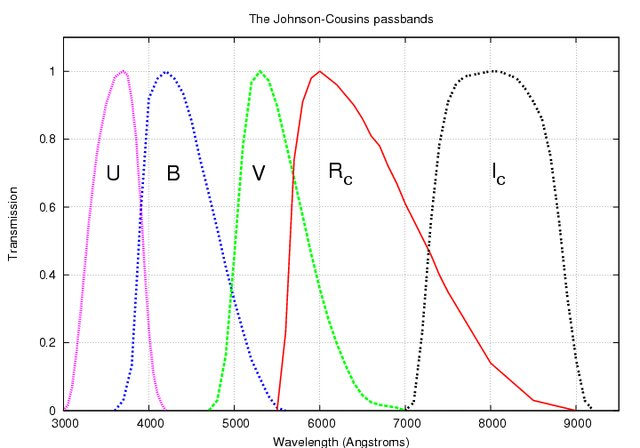
\includegraphics[width=\linewidth]{Figures/filter_curves.jpg}
    \caption{Καμπύλες διαπερατότητας για το σύστημα φίλτρων Johnson-Cousins. Ο άξονας y δείχνει την \textit{διαφάνεια}. Το φίλτρο V (visual) αφήνει να καταγραφούν τα ίδια φωτόνια (πάνω-κάτω) με αυτά που αντιλαμβάνονται τα μάτια μας. Δηλαδή με άλλα λόγια, η καμπύλη φασματικής ευαισθησίας του φίλτρου V είναι παρόμοια μ' εκείνη του ματιού μας.}
    \label{fig:filter_curves}
\end{figure}

Όταν παρατηρούμε ένα αστέρι μέσω ενός φίλτρου (π.χ. το V) τότε εμείς μετράμε:
\begin{equation}
    F_V = \int_0^{\infty} F(\lambda) S_V(\lambda) d\lambda
\end{equation}
όπου $F(\lambda)$ είναι το φάσμα που επέμπει ο αστέρας, και $S_V(\lambda)$ είναι η καμπύλη φασματικής ευαισθησίας, του φίλτρου και του ανιχνευτή.

Έτσι, μπορούμε να ορίσουμε τα μεγέθη ενός αστέρα στα διάφορα φίλτρα ως εξής:
\begin{eqnarray*}
    V \equiv m_V = -2.5 \log \left( \frac{F_V}{F_{V,0}} \right) = 2.5 \log F_{V,0} - 2.5 \log F_V = C_V - 2.5 \log F_V \\\\
    B \equiv m_B = -2.5 \log \left( \frac{F_B}{F_{B,0}} \right) = 2.5 \log F_{B,0} - 2.5 \log F_B = C_B - 2.5 \log F_B \\\\
    U \equiv m_U = -2.5 \log \left( \frac{F_U}{F_{U,0}} \right) = 2.5 \log F_{U,0} - 2.5 \log F_U = C_U - 2.5 \log F_U 
\end{eqnarray*}
όπου οι σταθερές $C_V, C_B, C_U$ κτλ ορίζονται με βάση τη φωτεινότητα του Vega στα αντίστοιχα μήκη κύματος, δηλαδή:
\begin{eqnarray*}
    C_V  &=& 2.5 \log(F_{V, Vega}) \\\\
    C_B  &=& 2.5 \log(F_{B, Vega}) \\\\
    C_U  &=& 2.5 \log(F_{U, Vega}) \hspace{1cm} \text{κτλ}
\end{eqnarray*}
Αυτό σημαίνει ότι εξ' ορισμού ισχύει $\boxed{m_{V,Vega} = m_{B,Vega} = m_{U,Vega} = \dots = 0}$
\\
{\color{red} \hrule} 
Ε: Ποιό είναι το βολομετρικό μέγεθος ενός αστέρα αν υποθέσουμε ότι εκπέμπει μόνο στα U,B,V,R;
Α: Αν κάποιος υποθέσει ότι το συνολικό μέγεθος $m_{\text{bol}}$ είναι απλώς το άθροισμα των επιμέρους μεγεθών στα διάφορα φίλτρα, τότε είναι λάθος! Με άλλα λόγια: $$m_{\text{bol}} \neq m_U + m_B + m_V + m_R$$
γιατί το μέγεθος είναι λογαριθμική ποσότητα. Αυτό που ισχύει είναι ότι η \textit{συνολική ροή θα ισούται με το άθροισμα των ροών στα αντίστοιχα φίλτρα}. Έτσι, αν γνωρίζουμε τα $m_U, m_B$ κτλ και θέλουμε να βρούμε το $m_{\text{bol}}$ dουλεύουμε ως εξής:
$$m_B = -2.5 \log \left( \frac{F_B}{F_{B,0}} \right) \Rightarrow -0.4m_B = \log \left( \frac{F_B}{F_{B,0}} \right) \Rightarrow F_B = F_{B,0} 10^{-0.4m_B}$$
Παρόμοια βρίσκουμε και τα $F_U, F_V, F_R$ και άρα $F_{\text{bol}} = F_B+F_V+F_U+F_R$. Τελικά $$m_{\text{bol}} = -2.5 \log \left( \frac{F_{\text{bol}}}{F_0} \right)$$
{\color{red} \hrule} 

Ο υπολογισμός της συνολικής φωτεινότητας ενός αστέρα είναι ο λόγος που κάνουμε παρατηρήσεις με περισσότερα από ένα φίλτρα. Παρόλα αυτά, υπάρχει και ένας άλλος τρόπος υπολογισμού, μέσω του $m_V$ και μόνο. Για αυτό τον λόγο θα πρέπει να ορίσουμε μία νέα ποσότητα η οποία είναι γνωστή ως \textit{βολομετρική διόρθωση} (bolometric correction) ή αλλιώς συντελεστής συνολικής διόρθωσης ως εξής:
\begin{equation}
    \boxed{BC = m_{\text{bol}} - m_V = M_{\text{bol}} - M_V}
\end{equation}

Η ιδέα για το BC είναι ότι {\color{blue}μπορεί να υπολογιστεί θεωρητικά}. Γνωρίζοντας ότι για τα περισσότερα άστρα το φάσμα τους προσαρμόζεται αρκετά ικανοποιητικά από το φάσμα ενός μέλανος σώματος, αν εγώ ξέρω τη θερμοκρασία ενός αστέρα, άρα ξέρω και το φάσμα του μέλανος σώματος που αντιστοιχεί σε αυτή τη θερμοκρασία, μπορώ να ολοκληρώσω το φάσμα ως προς όλα τα μήκη κύματος για να βρω την ολική λαμπρότητα του αστέρα, να ολοκληρώσω μετά το φάσμα μόνο στην περιοχή του φίλτρου V, και να υπολογίσω θεωρητικά τη ποσότητα BC για διάφορες θερμοκρασίες.

Άρα, παρατηρώντας το $m_V$ ενός αστέρα, μπορούμε να προσθέσουμε το BC που αντιστοιχεί στη θερμοκρασία του αστέρα (το οποίο έχει υπογισθεί θεωρητικά) και έτσι έχουμε μία εκτίμηση για το ολικό μέγεθος του αστέρα.
\\
{\color{red} \hrule}
\textbf{Για τον Ήλιο}: $M_{\text{bol}} = 4.74$ και $M_V = 4.83$. Άρα, $BC = -0.09$.
Παρατηρούμε ότι ο BC πρέπει πάντα να είναι αρνητικός καθώς τα μεγέθη ορίζονται με ένα μείον (μικρότερο μέγεθος συνεπάγεται πιο φωτεινός ο αστέρας).

\textbf{Για αστέρια με $T_{\text{eff}} \simeq 6700 \ \text{K}$} έχουμε $BC \simeq 0$. Αυτό σημαίνει ότι το $\lambda_{\text{max}}$ που αντιστοιχεί σε αυτή τη θερμοκρασία, δηλαδή το μεγαλύτερο μέρος της εκπεμπόμενης ακτινοβολίας διέρχεται μέσω του φίλτρου V.

\textbf{Για αστέρια με $T_{\text{eff}} > 6700 \ \text{K}$} το $\lambda_{\text{max}}$ μετατοπίζεται σε μικρότερα μήκη κύματος και άρα ``χάνουμε'' φωτόνια από εκεί.

\textbf{Για αστέρια με $T_{\text{eff}} < 6700 \ \text{K}$} αντίστοιχα, ``χάνουμε'' φωτόνια από τα μεγαλύτερα μήκη κύματος.
{\color{red} \hrule}

\underline{Παρατήρηση}: Βολομετρική διόρθωση μπορεί να οριστεί και σε άλλα μήκη κύματος πέρα του ορατού. Για παράδειγμα, σε μερικά ψυχρά άστρα όπου το μέγιστο της ενέργειάς τους εκπέμπεται στα υπέρυθρα μήκη κύματος, μπορούμε να εφαρμόσουμε ένα διαφορετικό σύνολο βολομετρικών διορθώσεων στο απόλυτο μέγεθος στα υπέρυθρα, αντί για το απόλυτο μέγεθος στα ορατά μήκη κύματος. Έτσι, $BC_K = M_{\text{bol}} - M_K$, όπου $BC_K$ και $M_K$ είναι η βολομετρική διόρθωση και το απόλυτο μέγεθος στην K-band αντίστοιχα.  
\hrule

Αφού λοιπόν θα μας αρκούσαν παρατηρήσεις μόνο σε ένα φίλτρο για να υπολογίσουμε τη συνολική φωτεινότητα ενός αστέρα, προκύπτει η εύλογη απορία τι μας χρειάζεται να παρατηρούμε στα άλλα φίλτρα. Η απάντηση είναι επειδή θέλουμε να υπολογίσουμε την επιφανειακή θερμοκρασία, $T_{\text{eff}}$ ενός αστέρα (χωρίς να χρειαστεί να έχουμε το συνολικό φάσμα του αστέρα), γνώση που είναι απαραίτητη για να βρούμε το BC.

\begin{figure}[h]
    \centering
    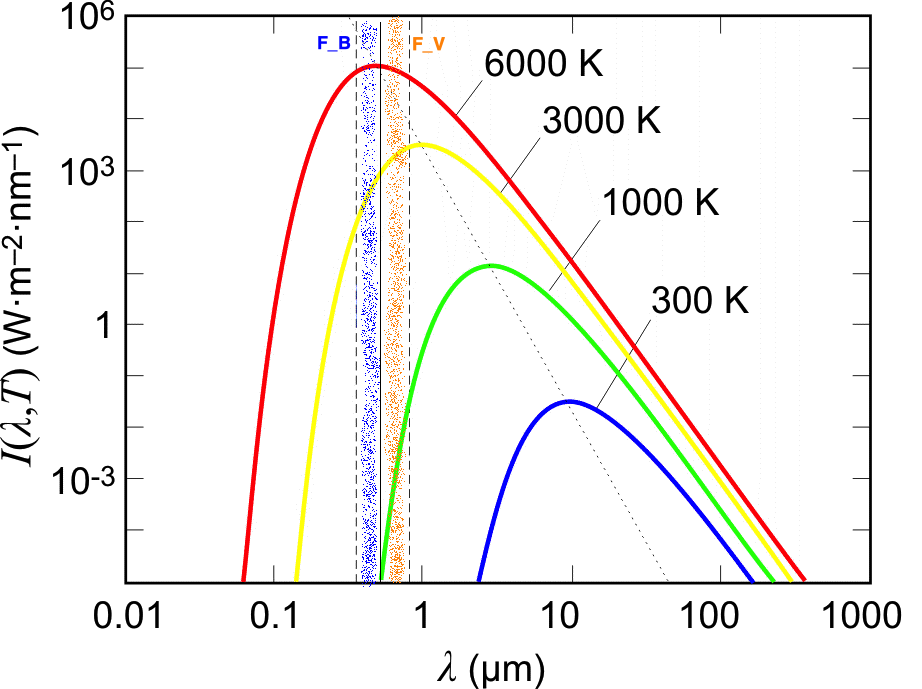
\includegraphics[width=\linewidth]{Figures/Planck_law_log_log_scale.png}
    \caption{Φάσματα μέλανων σωμάτων για διάφορες θερμοκρασίες. Το διάγραμμα είναι σε λογαριθμικούς άξονες γι' αυτό η μορφή των καμπυλών είναι διαφορετική.}
    \label{fig:planck_law_log_scale}
\end{figure}

Στο διάγραμμα \ref{fig:planck_law_log_scale} απεικονίζεται --ποιοτικά-- το εύρος των συχνοτήτων που καλύπτει το φίλτρο B (με μπλε χρώμα), ενώ με πορτοκαλί φαίνεται το εύρος συχνοτήτων που καλύπτει το φίλτρο V. {\color{blue} Άρα, η ροή του αστέρα στο φίλτρο B θα είναι το εμβαδόν της επιφάνειας που ορίζεται κάτω από την καμπύλη καθώς από τον ορισμό ξέρουμε ότι είναι το ολοκλήρωμα ως προς τα μήκη κύματος επι τη φασματική ευαισθησία του φίλτρου. Λόγω της μορφής των καμπυλών τα εμβαδά αυτά δεν είναι σταθερά}.

Αυτό που μας ενδιαφέρει είναι το εμβαδόν (η ροή) και στα δύο φίλτρα. Αν πάρουμε ως παράδειγμα το μέλαν σώμα θερμοκρασίας 6000 Κ, παρατηρούμε ότι το εμβαδόν στο B φίλτρο είναι ελαφρώς μεγαλύτερο από το εμβαδόν στο V φίλτρο. Άρα η διαφορά στα μεγέθη $B - V \equiv m_B - m_V < 0$ καθώς $F_B > F_V$.
Για το μέλαν σώμα θερμοκρασίας 3000 Κ, το εμβαδόν στο V φίλτρο είναι μεγαλύτερο από το εμβαδόν στο B φίλτρο. Άρα $B - V > 0$ καθώς $F_B < F_V$.
{\color{red} Η διαφορά στα μεγέθη των δύο φίλτρων δεν θα έχει το ίδιο πρόσημο! Έτσι, μετρώντας τη ροή του αστέρα σε δύο φίλτρα και παίρνοντας τη διαφορά στα μεγέθη τους, μπορούμε να υπολογίσουμε τη θερμοκρασία του αστέρα.}

\underline{Για να συνοψίσουμε}:\\
Χρειαζόμαστε παρατηρήσεις σε 2 τουλάχιστον φίλτρα. Παίρνοντας την διαφορά $B - V$, $U - V$ κτλ, βρίσκουμε τη θερμοκρασία του αστέρα. Γνωρίζοντας τη θερμοκρασία, έχουμε μία τιμή για τη βολομετρική διόρθωση που χρειαζόμαστε και κατά συνέπεια μπορούμε να υπολογίσουμε τη συνολική λαμπρότητα του αστέρα (αν γνωρίζουμε την απόσταση).

Αυτές οι διαφορές στα μεγέθη (π.χ. $B - V$) ονομάζονται ``\textit{δείκτες χρώματος}'' και συνήθως ορίζονται ως η διαφορά μεγέθους σε μικρότερο μήκος κύματος μείον το μέγεθος σε μεγαλύτερο μήκος κύματος. Συνηθισμένοι δείκτες χρώματος είναι οι $$B - V \equiv m_B - m_V, U - B \equiv m_U - m_B, V - R \equiv m_V - m_R$$

Θεωρώντας ότι ένα αστέρι εκπέμπει ως μέλαν σώμα, μπορούμε για κάθε θερμοκρασία να υπολογίσουμε θεωρητικά τι δείκτη χρώματος περιμένουμε. Στην πράξη, χρησιμοποιούμε διάφορες εμπειρικές σχέσεις όπως την παρακάτω για τον δείκτη $B-V$: 
\begin{equation}
    T_{\text{eff}} = \frac{9000 \ \text{K}}{(B - V) + 0.93}
\end{equation}
που ισχύει για αστέρια με δείκτη χρώματος $-0.1 \leq B-V \leq 1.4$ ή ισοδύναμα $4000 \ \text{K} \leq T_{\text{eff}} \leq 11000 \ \text{K}$.

\begin{itemize}
    \item Για τον Vega, $T_{\text{eff}} \approx 10000 \ \text{K}$ και εξ' ορισμού $B-V = U-B = \dots = 0$.
    \item Για αστέρια με $T_{\text{eff}} > 10000 \ \text{K} \longrightarrow B-V < 0$, ενώ για αστέρια με $T_{\text{eff}} < 10000 \ \text{K} \longrightarrow B-V > 0$. Αυτό το συμπέρασμα προκύπτει εύκολα αν σκεφτούμε ότι μεγαλύτερη θερμοκρασία συνεπάγεται $\lambda_{\text{max}}$ σε μικρότερη μήκη κύματος και άρα $F_B > F_V \Rightarrow m_B < m_V \Rightarrow B-V < 0$. Αντίστοιχη λογική ακολουθείται και για όταν $T_{\text{eff}} < 10000 \ \text{K}$.
\end{itemize}


\textbf{Ας υποθέσουμε ότι έχουμε ένα αστέρι ψυχρότερο από τον Vega και ότι ισχύει $\displaystyle \frac{F_B}{F_V} < \left( \frac{F_B}{F_V} \right)_{Vega}$. Να δείξετε ότι σε αυτή την περίπτωση $B-V > 0$.}

Γνωρίζουμε ότι 
\begin{eqnarray*}
\frac{F_B}{F_V} &<& \frac{F_{B,Vega}}{F_{V,Vega}} \Rightarrow \log \left( \frac{F_B}{F_V} \right) < \log \left( \frac{F_{B,Vega}}{F_{V,Vega}} \right) \Rightarrow \\\\\
&\Rightarrow & - \log \left( \frac{F_B}{F_V} \right) > - \log \left( \frac{F_{B,Vega}}{F_{V,Vega}} \right) \Rightarrow \\\\
&\Rightarrow & - 2.5 \log \left( \frac{F_B}{F_V} \right) > - 2.5 \log \left( \frac{F_{B,Vega}}{F_{V,Vega}} \right) \Rightarrow \\\\
&\Rightarrow & - \log \left( \frac{F_B}{F_V} \right) + \log \left( \frac{F_{B,Vega}}{F_{V,Vega}} \right) > 0 \Rightarrow \\\\
&\Rightarrow & {\color{green} -2.5 \log F_B} + {\color{purple} 2.5 \log F_V} + {\color{green} 2.5 \log F_{B,Vega}} {\color{purple} - 2.5 \log F_{V,Vega}} > 0 \Rightarrow \\\\
&\Rightarrow & -2.5 \left( \log F_B - \log F_{B,Vega} \right) + 2.5 \left( \log F_V - \log F_{V,Vega} \right) > 0 \Rightarrow \\\\
&\Rightarrow & \underbrace{-2.5 \log \left( \frac{F_B}{F_{B,Vega}} \right)}_{m_B} + \underbrace{2.5 \log \left( \frac{F_V}{F_{V,Vega}} \right)}_{- m_V} > 0 \Rightarrow \\\\
&\Rightarrow & m_B - m_V > 0 \Rightarrow \boxed{B - V > 0}
\end{eqnarray*}
\hrule 

Υπάρχει όμως λόγος να μελετάμε τα άστρα σε παραπάνω από 2 φίλτρα; Η απάντηση είναι πως ναι, καθώς μέχρι τώρα υποθέσαμε ότι δεν παρεμβάλεται τίποτα μεταξύ του παρατηρητή και του αστέρα. Στην πραγματικότητα, και ιδιαίτερα για τα άστρα που βρίσκονται στο γαλαξιακό επίπεδο, υπάρχουν αέρια και σκόνη που απορροφούν μέρος του φωτός.

Η απορρόφηση του οπτικού φωτός από τη μεσοαστρική σκόνη γίνεται με διαφορετικό τρόπο στα διάφορα μήκη κύματος. Η απορρόφηση είναι μεγαλύτερη στα μικρότερα μήκη κύματος (στο ``μπλε'' φως) οπότε τα αστέρια εμφανίζονται περισσότερο κόκκινα απ 'οτι είναι στην πραγματικότητα. Αυτό το φαινόμενο ονομάζεται ``\textit{μεσοαστρική ερυθρή χρώση}'' (interstellar reddening). Αν όμως έχουμε μετρήσεις του μεγέθους των αστέρων σε διάφορα φίλτρα, τότε μπορούμε να υπολογίσουμε την απορρόφηση στα διάφορα μήκη κύματος, να διορθώοσυμε τους παρατηρούμενες δείκτες χρώματος, και άρα να υπολογίσουμε τη σωστή $T_{\text{eff}}$ και τον συντελεστή βολομετρικής διόρθωσης BC.


Λόγω του φαινομένου της μεσοαστρικής ερυθρής χρώσης, ένας αστέρας παρατηρείται πιο κόκκινος απ' ότι είναι στην πραγματικότητα, δηλαδή με αλλοιωμένο δείκτη χρώματος. Αν $(B-V)$ είναι ο παρατηρούμενος και $(B-V)_0$ ο πραγματικός δείκτης χρώματος, τότε η διαφορά τους
\begin{equation}
    E_{(B-V)} = (B-V) - (B-V)_0
\end{equation}
ονομάζεται ``\textit{υπεροχή χρώματος}'' (color excess). Από την υπεροχή χρώματος υπολογίζεται τελικά η απορρόφηση σε αστρικά μεγέθη ($A_{\text{V}}$ για το οπτικό και $A_{\text{B}}$ για το κυανό) από τις εμπειρικές σχέσεις
\begin{align}
    A_{\text{V}} & = 3 E_{(B-V)} \\\nonumber\\
    A_{\text{B}} & = 4 E_{(B-V)}
\end{align}


\section{Φασματική ανάλυση}
Στα μέσα του 19ου αιώνα οι Kirchhoff και Bunsen παρατήρησαν ότι τα φάσματα των φυσικών σωμάτων ακολουθούν τους εξής δύο γενικούς κανόνες:
\begin{enumerate}
    \item Τα στερεά και τα υγρά σώματα εκπέμπουν συνεχές φάσμα, ενώ τα (αραιά) αέρια εκπέμπουν γραμμικό φάσμα.
    \item Όταν ένα αέριο παρεμβάλλεται μεταξύ μιας (θερμότερης από αυτό) πηγής συνεχούς φάσματος και του παρατηρητή, δημιουργούνται γραμμές απορρόφησης στο συνεχές φάσμα. Οι γραμμές αυτές έχουν το ίδιο μήκος κύματος με τις γραμμές εκπομπής του φάσματος του αερίου του κανόνα (1).
\end{enumerate}

Σε αυτό το κεφάλαιο θα αναλύσουμε κάποια χαρακτηριστικά των αστρικών φασμάτων δίνοντας έμφαση στο σχηματισμό της γραμμικής συνιστώσας, ενώ το πως μια αέρια μάζα --όπως ένας αστέρας-- μπορεί να έχει και συνεχές φάσμα, που έρχεται σε αντίθεση με τον κανόνα (1), θα γίνει αντιληπτό στο επόμενο κεφάλαιο.

\subsection{Αστρικά φάσματα}

Μπορούμε να πάρουμε το φάσμα μιας πηγής χρησιμοποιώντας ένα πρίσμα ή ένα φράγμα περίθλασης. Παρόλο που η λειτουργία των δύο αυτών οργάνων βασίζεται σε εντελώς διαφορετικά φυσικά φαινόμενα, τα αποτελέσματα που μας δίνουν είναι τα ίδια: αναλύουν μία παράλληλη πολυχρωματική δέσμη φωτός, σε μία αποκλίνουσα δέσμη, σε κάθε διεύθυνση της οποίας αντιστοιχεί φως μια συγκεκριμένης συχνότητας. Στη συνέχεια το φάσμα καταγράφεται φωτογραφικά ή φωτοηλεκτρικά.

Το φάσμα μιας πηγής χωρίζεται σε δύο συνιστώσες: τη \textbf{συνεχής} συνιστώσα και τη \textbf{γραμμική} συνιστώσα. Η τελευταία αποτελείται από \textbf{φασματικές γραμμές}, δηλαδή στενές φασματικές περιοχές πλάτους $\Delta \lambda$, όπου $\Delta \lambda \ll \lambda$, στις οποίες η φωτεινή ένταση έχει τιμή πολύ μεγαλύτερη (φωτεινές γραμμές) ή πολύ μικρότερη (σκοτεινές γραμμές) από τη μέση τιμή των γειτονικών της περιοχών.
Η συνεχής συνιστώσα αποτελείται από την εξομαλυμένη καμπύλη που προκύπτει αν ``αφαιρέσουμε'' από το φάσμα τις φασματικές γραμμές, ή αν ``προσαρμόσουμε'' στην πειραματική καμπύλη του φάσματος μια συνεχής ``θεωρητική'' καμπύλη σύμφωνα με κάποιο λογικό κριτήριο. Τέτοια θεωρητική καμπύλη μπορεί να είναι για παράδειγμα μία καμπύλη Planck (μέλανος σώματος) αν έχουμε λόγους να πιστεύουμε ότι το φωτοβόλο σώμα εκπέμπει θερμικά\footnote{Θερμική ακτινοβολία είναι η ακτινοβολία που εκπέμπεται από ένα σώμα λόγω της θερμικής του κατάστασης και η έντασή της περιγράφεται από τον νόμο του Planck.} και βρίσκεται σε θερμοδυναμική ισορροπία, ένα πολυώνυμο αν πιστεύουμε ότι το σώμα εκπέμπει ακτινοβολία σύγχροτρον\footnote{Ακτινοβολία σύγχροτρον είναι η ακτινοβολία που εκπέμπεται όταν ηλεκτρόνια με σχετικιστικές ταχύτητες κινούνται μέσα σε μαγνητικό πεδίο. Η ακτινοβολία αυτή δημιουργεί συνεχές φάσμα και εκπέμπεται μέσα στα όρια ενός στενού κώνου γωνίας $\alpha = 2m_0 c^2/E$, με άξονα κάθετο στη διεύθυνση του μαγνητικού πεδίου, όπου $m_0$ η μάζα ηρεμίας του ηλεκτρονίου και $E$ η ενέργειά του.} ή ακόμη και αυτή που προκύπτει από μία απλή γραφική εξομάλυνση των δεδομένων.

Η συνεχής συνιστώσα των φασμάτων των αστέρων μοιάζει πολύ με το φάσμα μέλανος σώματος, εφόσον ως θερμοκρασία του αστέρα πάρουμε την ενεργό θερμοκρασία του (σχήμα \ref{fig:continuous_spectra}). Οι αποκλίσεις της συνεχούς συνιστώσας από το μέλαν σώμα οφείλονται στο γεγονός ότι η ακτινοβολία προέρχεται από διάφορα βάθη, με διάφορες θερμοκρασίες. Αυτό σημαίνει ότι το συνεχές φάσμα μοιάζει να είναι μια σύνθεση φασμάτων πολλών μελανών σωμάτων διαφορετικών θερμοκρασιών. Επίσης, στη φωτόσφαιρα του άστρου παρουσιάζονται αποκλίσεις από τη θερμοδυναμική ισορροπία που προϋποθέτει ο νόμος του Planck και παρουσιάζει σημαντική διαφάνεια (δεν επικρατεί θερμοδυναμική ισορροπία σε όλο το εξωτερικό στρώμα του αστέρα από το οποίο προέρχεται η ακτινοβολία).

\begin{figure}[h]
    \centering
    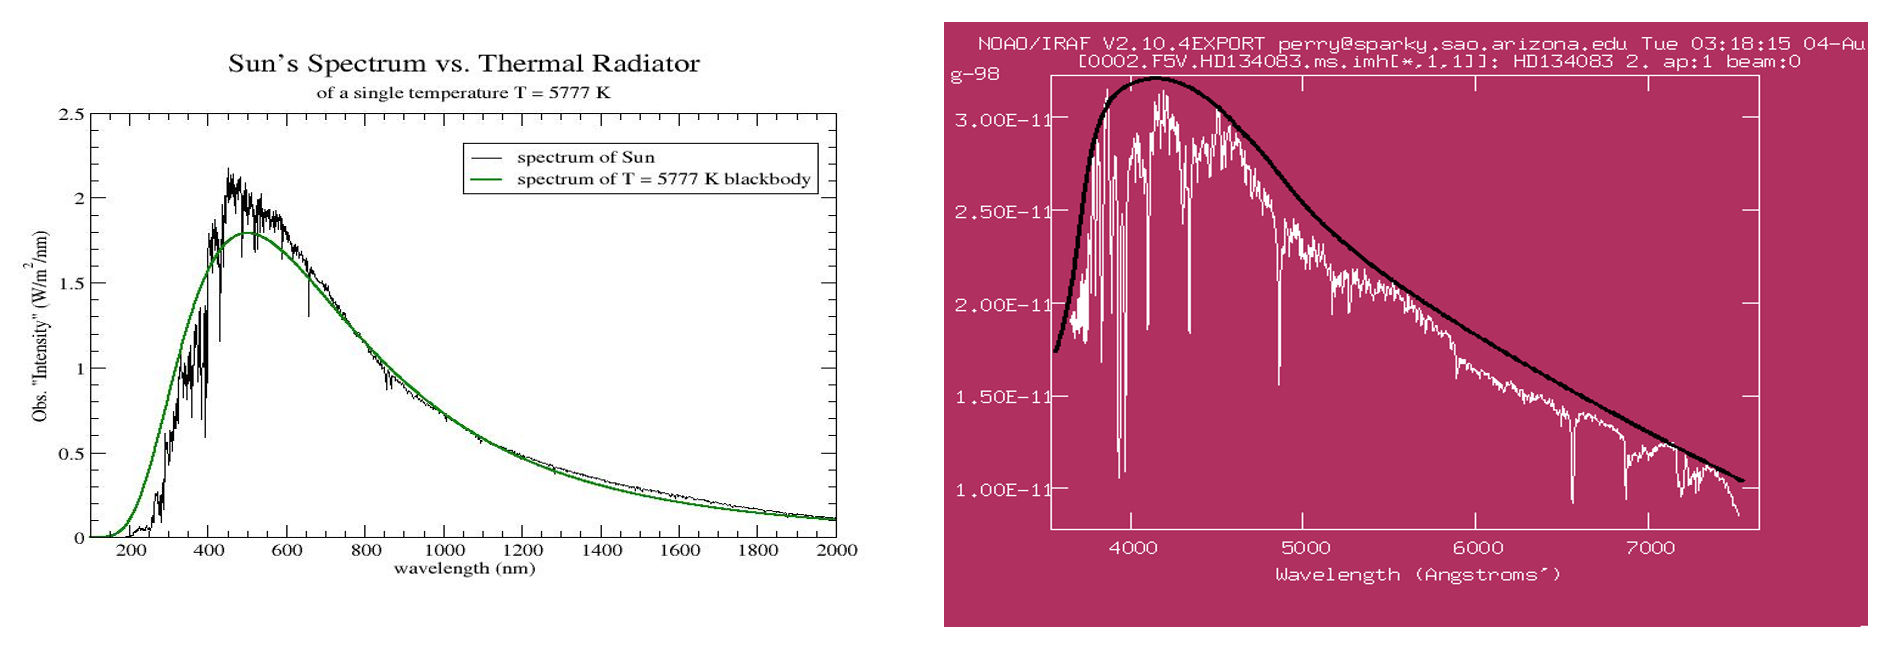
\includegraphics[width=\linewidth]{Figures/contin_spectra.png}
    \caption{\textbf{Αριστερά:} Προσαρμογή συνεχούς φάσματος θερμοκρασίας $ T \sim 5777 \ K$ στο φάσμα του Ήλιου. \textbf{Δεξιά:} Προσαρμογή συνεχούς φάσματος θερμοκρασίας $ T \sim 6660 \ K$ στο φάσμα του αστέρα HD134083. Και στις δύο περιπτώσεις είναι χαρακτηριστική η παρουσία φασματικών γραμμών απορρόφησης.}
    \label{fig:continuous_spectra}
\end{figure}

Επειδή το πλάτος $\Delta \lambda$ των φασματικών γραμμών είναι συνήθως πολύ μικρό συγκρικά με το πλάτος της οπτικής περιοχής, η φωτεινή ενέργεια που αντιστοιχεί σ' αυτές είναι πολύ μικρή, έστω κι αν η έντασή τους είναι πολύ μεγαλύτερη (ή μικρότερη) από την τιμή της συνεχούς συνιστώσας στην οπτική περιοχή. Έτσι, η ύπαρξη των φασματικών γραμμών δεν επηρεάζει σημαντικά τη φωτεινότητα ενός αστέρα και κατ' επέκταση το μέγεθός του ($m_U, m_B, m_V$ κτλ). Παρόλα αυτά, η ένταση και το πλάτος των φασματικών γραμμών των αστρικών φασμάτων είναι φορείς που μας μεταφέρουν τις σημαντικότερες πληροφορίες που έχουμε σήμερα στη διάθεσή μας για του αστέρες: φυσικές συνθήκες στην επιφάνεια και την ατμόσφαιρά τους (πίεση και θερμοκρασία), χημική σύσταση, ταχύτητα περιστροφής, ακτινική ταχύτητα ως προς τον παρατηρητή. Για παράδειγμα, η μέτρηση της μετατόπισης του μήκους κύματος των φασματικών γραμμών από τα διάφορα τμήματα της επιφάνειας του αστέρα, προς μικρότερα ή μεγαλύτερα μήκη κύματος (λόγω φαινομένου Doppler) μας επιτρέπει τη μέτρηση της ακτινικής συνιστώστας της ταχύτητας του αστέρα. Αντίστοιχα, η μέτρηση του εύρους των φασματικών γραμμών μας επιτρέπει τον προσδιορισμό της γωνιακής ταχύτητας περιστροφής του αστέρα.Γενικά πάντως, η πεπλάτυνση των φασματικών γρμαμών οφείλεται σε πολλούς παράγοντες, όπως η θερμική κίνηση των συστατικών του αερίου. Σε αυτή την περίπτωση βέβαια, η πεπλάτυνση δεν είναι ίδια για όλες τις φασματικές γραμμές που αντιστοιχούν στα διάφορα χημικά στοιχεία παρόντα στην ατμόσφαιρα του αστέρα. Η ταχύτητα περιστροφής όμως επηρεάζει το εύρος όλων των φασματικών γραμμών το ίδιο.

Η δημιουργία της συνεχούς συνιστώσας του φάσματος αν και έχει θεωρητικό ενδιαφέρον, οι ιδιότητές της λίγο εξαρτώνται από το μηχανισμό παραγωγής της και κατ' επέκταση από τη χημική σύσταση του αστέρα.

\subsection{Σχηματισμός φασματικών γραμμών}
Οι φασματικές γραμμές δημιουργούνται όταν μεταβάλλεται η ενέργεια ενός ατόμου ή ενός μορίου (ή ελεύθερης ρίζας) μεταξύ κβαντισμένων ενεργειακών σταθμών. Στην περίπτωση των μορίων, αυτό συμβαίνει είτε όταν μεταβάλλεται το πλάτος της ταλάντωσης ή η σχετική θέση των ατόμων τους, είτε όταν μεταβάλλεται η στροφορμή τους. Η ενέργεια ενός ατόμου, από την άλλη μεριά, μεταβάλλεται όταν μεταβληθεί ένας από τους τέσσερις κβαντικούς αριθμούς που χαρακτηρίζουν την ενεργειακή κατάσταση ενός ηλεκτρονίου. Η μεταβολή αυτή της ενέργειας κατά $\Delta E$ μπορεί να γίνει είτε όταν το άτομο απορροφά ($\Delta E > 0$) είτε όταν εκπέμπει $\Delta E < 0$ ένα φωτόνιο συχνότητας $\nu$, η οποία δίνεται από τη σχέση $|\Delta E| = h\nu$, όπου $h$ η σταθερά του Planck.

Όταν από μια δέσμη Η/Μ ακτινονολίας, που αποτελείται από συνεχή κατανομή συχνοτήτων, απορροφώνται φωτόνια συχνότητας $\nu_0$, τότε στο παρατηρούμενο φάσμα της δημιουργείται μία \textit{γραμμή απορρόφησης}. Όταν προστίθενται φωτόνια συχνότητας $\nu_0$, τότε στο φάσμα της επιπροστίθεται μία \textit{γραμμή εκπομπής}. Το αν η φασματική γραμμή που δημιουργείται σε κάθε περίπτωση θα είναι γραμμή εκπομπής ή απορρόφησης εξαρτάται από τη θερμοδυναμική κατάσταση της ύλης, δηλαδή των ίδιων των ατόμων.

\begin{figure}[h]
    \centering
    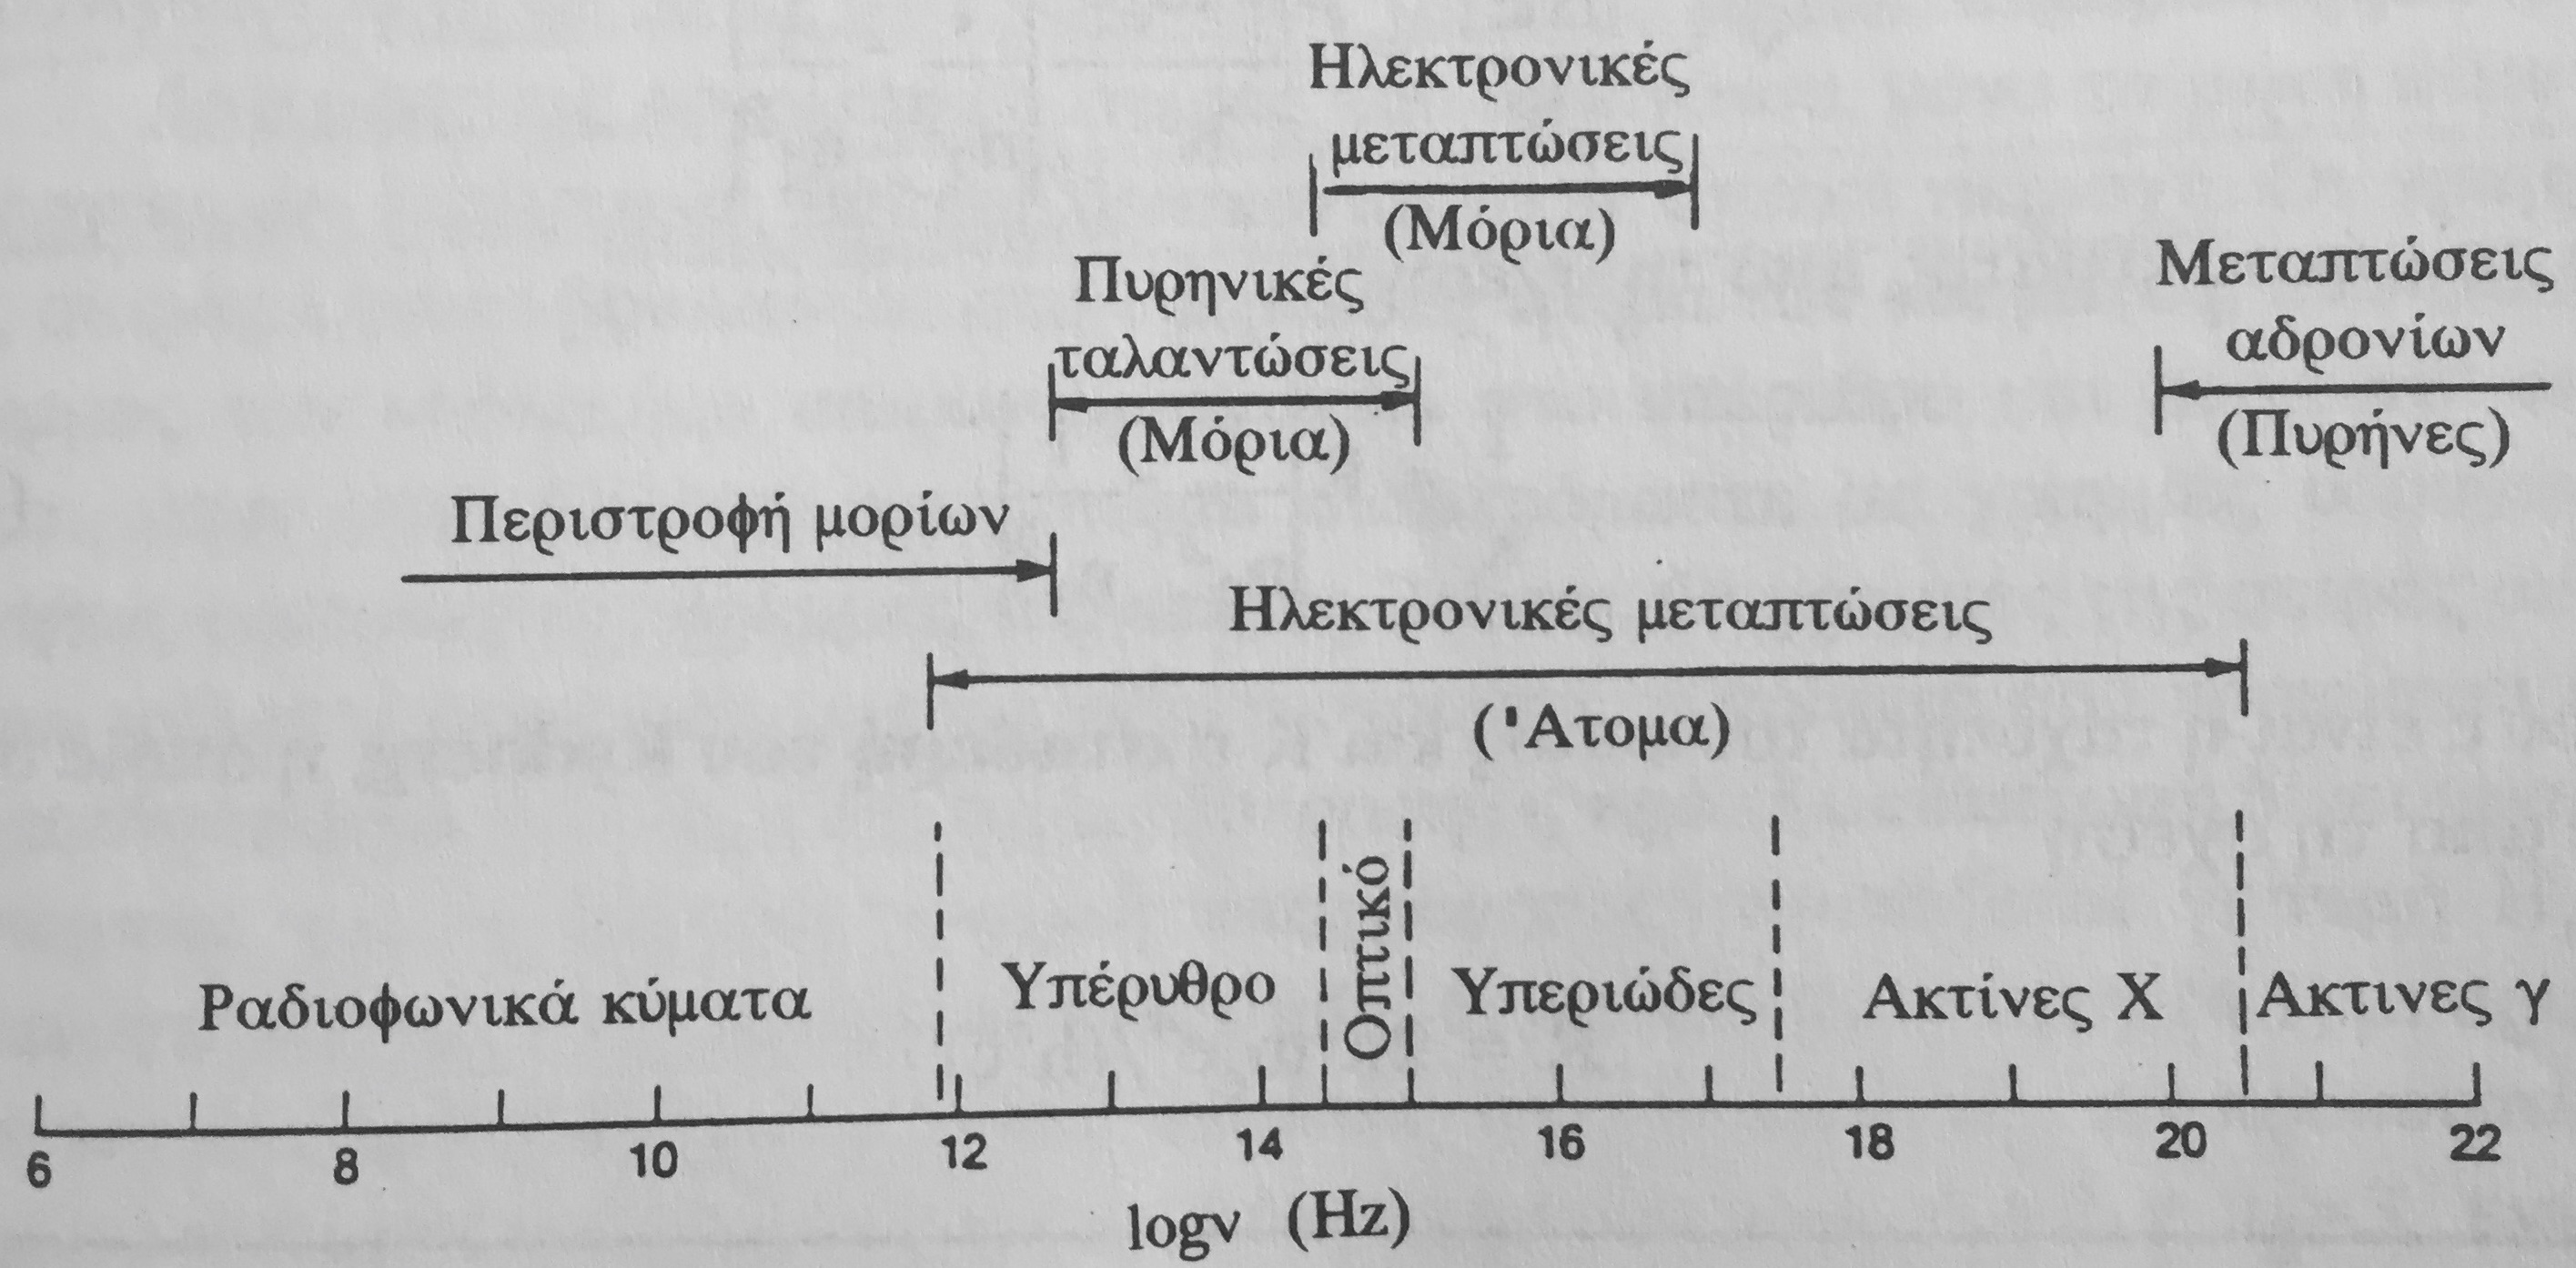
\includegraphics[width=\linewidth]{Figures/energy_transitions.jpeg}
    \caption{Ενεργειακές μεταπτώσεις στις οποίες οφείλονται η δημιουργία φασματικών γραμμών.}
    \label{fig:energy_transitions}
\end{figure}

\subsubsection{Φασματικές σειρές του Υδρογόνου}
Για λόγους απλότητας, θα θεωρήσουμε ότι η μοναδική αιτία αλλαγής της ενεργειακής κατάστασης ενός ατόμου είναι η μετάπτωση ενός ηλεκτρονίου από μία στοιβάδα σε μία άλλη, δηλαδή η αλλαγή του κύριου κβαντικού αριθμού, $(n = 1,2,3, \dots)$. Με άλλα λόγια, δεν θα μιλήσουμε καθόλου για ενεργειακές μεταπτώσεις μορίων ή ενεργειακές μεταπτώσεις υπέρλεπτης υφής (μεταπτώσεις που προκαλούνται λόγω της αλληλεπίδρασης του πυρήνα με το ηλεκτρονιακό νέφος, π.χ. γραμμή εκπομπής 21-cm του Υδρογόνου).

Το Υδρογόνο είναι με διαφορά το στοιχείο με τη μεγαλύτερη αφθονία τοσο στο σύμπαν όσο και στους αστέρες. Σε συνδυασμό με το γεγονός ότι είναι και το πιο εύκολα μελετήσιμο λόγω της απλής δομής του, τα αποτελέσματα αυτά είναι εξαιρετικά χρήσιμα.

Η ενέργεια του μοναδικού ηλεκτρονίου του ατόμου του Υδρογόνου δίνεται από τη σχέση
\begin{equation}
    E = - \frac{1}{n^2} \frac{2\pi^2 m_e e^4}{h^2}
\end{equation}
όπου $m_e$, $e$ και $n$ είναι η μάζα ηρεμίας, το φορτίο και ο κύριος κβαντικός αριθμός του ηλεκτρονίου αντίστοιχα.
Αν το ηλεκτρόνιο μεταβεί από μία στάθμη με κύριο κβαντικό αριθμό $n_i$ σε μία άλλη με κύριο κβαντικό αριθμό $n_f$, τότε η ενέργειά του μεταβάλλεται κατά 
\begin{equation}
    \Delta E = E_2 - E_1 = - \frac{2\pi^2 m_e e^4}{h^2} \left( \frac{1}{n_f^2} - \frac{1}{n_i^2} \right)
\end{equation}
Όταν $n_i < n_f$ τότε $\Delta E > 0 $, οπότε έχουμε απορρόφηση φωτονίου από το άτομο το οποίο μεταβαίνει από τη στάθμη χαμηλότερης ενέργειας ($n_i$) στη στάθμη υψηλότερης ενέργειας ($n_f$). Στην αντίθετη περίπτωση όπου $n_i > n_f$, έχουμε εκπομπή φωτονίου. Και στις δύο περιπτώσεις, η συχνότητα του φωτονίου δίνεται από τη σχέση

\begin{equation}
    \nu = \frac{|\Delta E|}{h} = \frac{2 \pi^2 m_e e^4}{h^3} \left| \frac{1}{n_f^2} - \frac{1}{n_i^2} \right|
\end{equation}
και το μήκος κύματος από τη σχέση του Rydberg

\begin{equation}
    \label{eq:rydberg_formula}
    \frac{1}{\lambda} = Z^2 R \left| \frac{1}{n_f^2} - \frac{1}{n_i^2} \right|
\end{equation}
όπου $Z$ είναι ο ατομικός αριθμός του ατόμου και $R$ η σταθερά του Rydberg η οποία δίνεται από τη σχέση $$R = \frac{2\pi^2 m_e e^4}{h^3 c}$$

Εφαρμόζοντας τη σχέση \eqref{eq:rydberg_formula} για το άτομο του Υδρογόνου ($Z=1$) τότε προκύπτουν οι εξής σειρές (δες και σχήμα \ref{fig:hydrogen_lines}):

\begin{itemize}
    \item Για $n_f = 1$ και $n_i=2,3, \dots$ τότε έχουμε τη σειρά \textit{εκπομπής Lyman}. Στην περίπτωση που $n_i = 1$ και $n_f = 2,3, \dots$ τότε έχουμε τη σειρά \textit{απορρόφησης Lyman}.
    \item Για $n_f = 2$ και $n_i=3,4, \dots$ τότε έχουμε τη σειρά εκπομπής Balmer. Στην περίπτωση που $n_i = 2$ και $n_f = 3,4, \dots$ τότε έχουμε τη σειρά απορρόφησης Balmer. Αυτή η σειρά είναι και η πιο σημαντική στην Οπτική Αστρονομία καθώς τα μήκη κύματος αυτής της σειράς βρίσκονται στην οπτική περιοχή. 
    
    Η γραμμή που προκύπτει από την μετάπτωση $n_i = 3 \rightarrow n_f = 2$ ονομάζεται γραμμή εκπομπής $H_{\alpha}$. Αντίστοιχα, η αντίστροφη μετάβαση $n_i = 2 \rightarrow n_f = 3$ ονομάζεται γραμμή απορρόφησης $H_{\alpha}$. Με την ίδια λογική μπορούμε να ορίσουμε τη γραμμή Balmer $H_{\beta}$ που αντιστοιχεί στην μετάβαση $n_i = 4 \rightarrow n_f = 2$ (ή το αντίστροφο), την γραμμή $H_{\gamma}$ για την μετάβαση $n_i = 5 \rightarrow n_f = 2$ κτλ.
    
    Το μήκος κύματος της σειρά Balmer ξεκινάει από $\lambda(H_{\alpha}) = 6563$Å και μειώνεται όσο αυξάνει η τάξη της γραμμής τείνοντας σε μια οριακή τιμή $\lambda(H_{\infty}) = 3546$Å. Στην περιοχή του οριακού αυτού μήκους κύματος οι γραμμές απορρόφησης είναι τόσο κοντά η μία με την άλλη, ώστε αλληλοεπικαλύπτονται με αποτέλεσμα το υπόβαθρο στην περιοχή αυτή να εμφανίζει μία ασυνέχεια, η οποία ονομάζεται \textbf{ασυνέχεια Balmer} και το ύψος της εξαρτάται από τη θερμοκρασία του αστέρα προσφέροντας έτσι ένα ακόμα παρατηρησιακό εργαλείο για τη μέτρησή της. 
    \item Για $n_f = 3$ και $n_i=4,5, \dots$ τότε έχουμε τη σειρά \textit{εκπομπής Paschen} (και αντίστροφα για την γραμμή απορρόφησης).
    \item Για $n_f = 4$ και $n_i=5,6, \dots$ τότε έχουμε τη σειρά \textit{εκπομπής Brackett} (και αντίστροφα για την γραμμή απορρόφησης).
    \item Για $n_f = 5$ και $n_i=6,7, \dots$ τότε έχουμε τη σειρά \textit{εκπομπής Pfund} (και αντίστροφα για την γραμμή απορρόφησης).
    \item Για $n_f = 6$ και $n_i=7,8, \dots$ τότε οι σειρές που προκύπτουν δεν έχουν κάποια συγκεκριμένη ονομασία.
\end{itemize}


\begin{figure}[h]
    \centering
    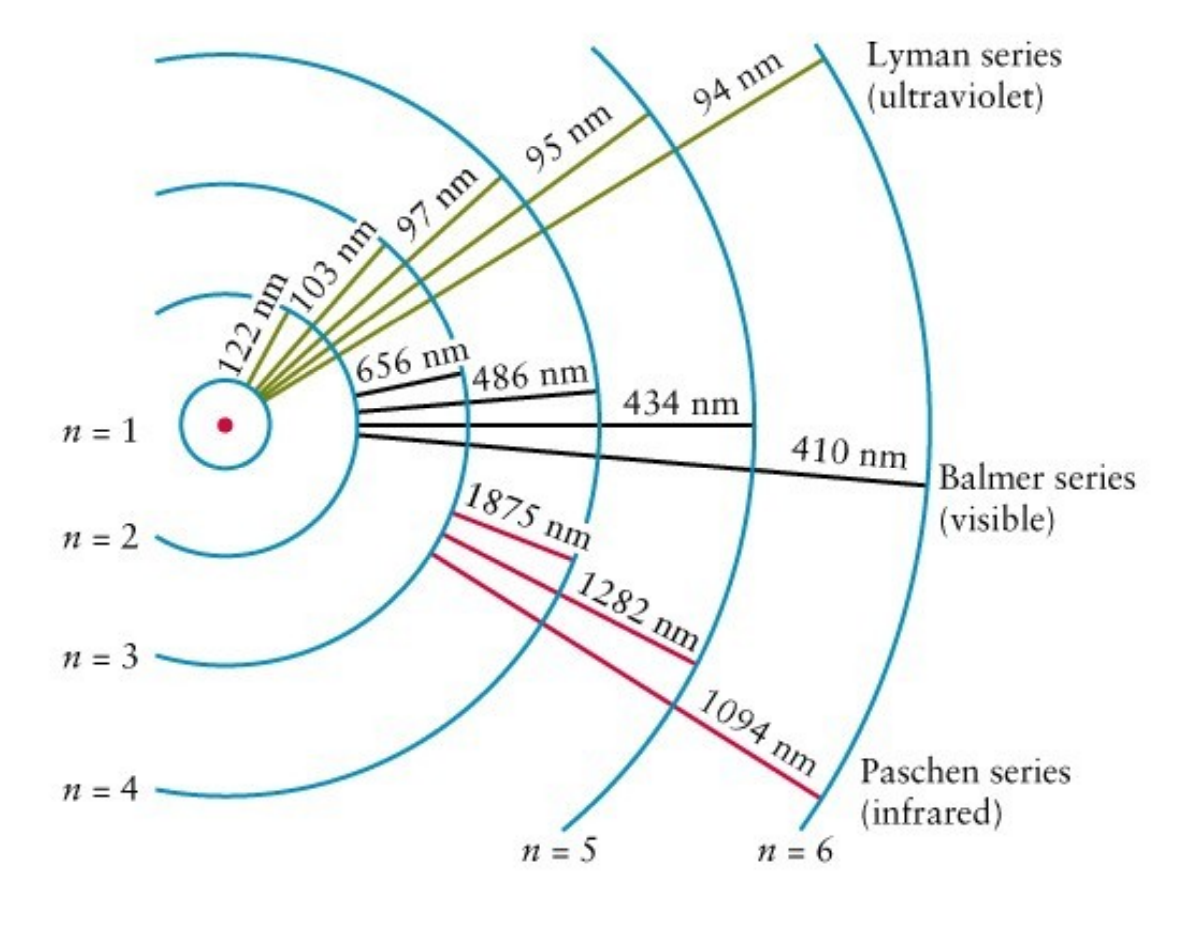
\includegraphics[scale=0.5]{Figures/hydrogen_spectral_lines.png}
    \caption{Σειρές Lyman, Balmer και Paschen για το άτομο του Υδρογόνου. Οι σειρές Brackett και Pfund, καθώς και άλλες ανώτερες σειρές, δεν παρουσιάζονται στο συγκεκριμένο διάγραμμα.}
    \label{fig:hydrogen_lines}
\end{figure}



\subsection{Φαινόμενο Zeeman}
Όταν τα άτομα στα οποία οφείλεται η δημιιουργία των φασματικών γραμμών βρίσκονται σε μαγνητικό πεδίο, τότε οι ενεργειακές τους στάθμες μεταβάλλονται, έτσι ώστε κάθε φασματική γραμμή διασπάται σε δύο, ή περισσότερες, πολωμένες συνιστώσες. Το φαινόμενο αυτό ονομάζεται ``φαινόμενο Zeeman'' (το ηλεκτρικό ανάλογο αυτού του φαινομένου είναι το φαινόμενο Stark όπου οι φασματικές γραμμές διασπόνται υπό την παρουσία ηλεκτρικού πεδίου) και επειδή η απόσταση των διάφορων συνιστωσών εξαρτάται από την ένταση του μαγνητικού πεδίου, το εκμεταλλευόμαστε για την μέτρηση αστρικών, μεσοαστρικών και γαλαξιακών μαγνητικών πεδίων. 

Στην απλούστερη περίπτωση (το ομαλό φαινόμενο Zeeman) μία φασματική γραμμή συχνότητας $\nu_{\circ}$ διασπάται σε τρεις συνιστώσες με συχνότητες $\nu_{\circ} - \Delta \nu$, $\nu_{\circ}$, και $\nu_{\circ} + \Delta \nu$. Αν η ένταση του μαγνητικού πεδίου, $B$, μετριέται σε Gauss, τότε η διαφορά συχνότητας $\Delta \lambda$, δίνεται απο τη σχέση 
\begin{equation}
    \Delta \nu =  \frac{eB}{4\pi m c} = 1.4 \times 10^6 \ B \ \ Hz
\end{equation}

Οι συσκευές μέτρησης των μαγνητικών πεδίων που βασίζονται σε παρατηρήσεις Η/Μ ακτινοβολίας ονομάζονται \textit{μαγνητογράφοι}. 



\section{Φασματική Ταξινόμηση}
Όπως είδαμε, Οι παράγοντες που καθορίζουν το φάσμα ενός αστέρα είναι η επιφανειακή θερμοκρασία ($ T_{eff}$), η ταχύτητα του αστέρα ($\boldsymbol{u}$), η γωνιακή ταχύτητα περιστροφής ($\boldsymbol{\omega}$), η ένταση του μαγνητικού πεδίου ($\boldsymbol{B}$), και η πίεση στην επιφάνεια του αστέρα. Τα αστρικά αυτά φάσματα κυριαρχούνται από γραμμές απορρόφησης (ορισμένα άστρα εμφανίζουν και αδύναμες γραμμές εκπομπής) με τις συνηθέστερες γραμμές απορρόφησης να είναι αυτές της σειράς Balmer του Υδρογόνου. Επειδή η ένταση των γραμμών απορρόφησης εξαρτάται άμεσα από την ενεργό θερμοκρασία του αστέρα, μπορούμε να ταξινομήσουμε τα αστέρια με βάση την ένταση των γραμμών απορρόφησης του Υδρογόνου και να καθορίσουμε με αυτό τον τρόπο την ενεργό θερμοκρασία τους.



\subsection{Ταξινόμηση κατα Harvard}
Αρχικά οι αστρονόμοι ταξινόμησαν τα αστρικά φάσματα αλφαβητικά σε φασματικούς τύπους (spectral types, Sp) με πρώτο κριτήριο την ένταση της γραμμής $H_{\alpha}$ της σειράς Balmer. Έτσι τα αστέρια τύπου Α είχαν την εντονότερη γραμμή $H_{\alpha}$, οι τύπου Β αστέρες είχαν λιγότερο έντονη γραμμή $H_{\alpha}$ κ.ο.κ.
Για τους αστέρες που είχαν τόσο ασθενή γραμμή $H_{\alpha}$, ώστε να μην μπορεί να χρησιμοποιηθεί ως κριτήριο ταξινόμησης, οι αστρονόμοι εισήγαγαν ως συμπληρωματικά κριτήρια την παρουσία ή την απουσία και άλλων φασματικών γραμμών (π.χ. ουδέτερα άτομα, ιόντα, μοριακές ταινίες).

Με την ανάλυση πολλών φασμάτων, διαπιστώθηκε ότι οι γραμμές απορρόφησης -εκτός του Υδρογόνου- δεν έδειχναν να μεταβάλλονται ομαλά από τον έναν φασματικό τύπο στον επόμενο. Αντίθετα, έδειχναν να εμφανίζονται και να εξαφανίζονται απότομα. Έτσι, οδηγήθηκαν στην αναδιάταξη της -αρχικά αλφαβητικής- ακολουθίας των φασματικών τύπων σε μία νέα ακολουθία όπου το χαρακτηριστικό της ήταν η συνεχής και μονότονη μεταβολή της ενεργού θερμοκρασίας. Η φασματική ταξινόμηση που προέκυψε ονομάστηκε ταξινόμηση κατα Harvard (σχήμα \ref{fig:spectral_classes_harvard}) επειδή προτάθηκε από ερευνητές του Πανεπιστημίου του Harvard.

Κάθε φασματικός τύπος της συγκεκριμένης ταξινόμησης διαιρείται σε δέκα υποκατηγορίες που χαρακτηριζόνται από τους αριθμούς $0,1,2,\dots , 9$. Ένα αστέρι φασματικού τύπου $ F1$ είναι πιο θερμό από ένα αστέρι $ F3$ αλλά πιο ψυχρό από ένα αστέρι $ A9$. Έτσι, οι θερμότεροι αστέρες που έχουν παρατηρηθεί μέχρι σήμερα είναι αστέρες φασματικού τύπου $ O5$ $ T_{eff} = 50000 \ K$, ενώ οι ψυχρότεροι αστέρες (ερυθροί νάνοι) είναι φασματικού τύπου $ M9$ με $ T_{eff} = 2900 \ K$. Ένας γενικός μνημονικός κανόνας για την συγκεκριμένη ταξινόμηση είναι 
\begin{center}
    \textbf{O}h, \textbf{B}e \textbf{A} \textbf{F}ine \textbf{G}irl/\textbf{G}uy, \textbf{K}iss \textbf{M}e
\end{center}


\begin{figure}[h]
    \centering
    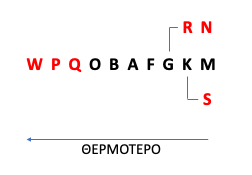
\includegraphics[scale=0.6]{Figures/spectral_classes.png}
    \caption{Φασματική ταξινόμηση κατά Harvard βάσει την ενεργό θερμοκρασία των άστρων. Κάθε τύπος αποτελείται από 10 υποκατηγορίες από το 0 εώς το 9. Οι τύποι P και Q δεν είναι απαραίτητο να ακολουθούν την μονότονη αύξηση της επιφανειακής θερμοκρασίας βάσει της οποίας ταξινομούνται τα αστέρια στους υπόλοιπους τύπους.}
    \label{fig:spectral_classes_harvard}
\end{figure}

Όπως φαίνεται και στο σχήμα \ref{fig:spectra_comparisson_table}, η ένταση των γραμμών Balmer ξεκινάει σχεδόν από το μηδεν ($ Sp = O5$), φτάνει σε κάποιο μέγιστο ($ Sp = A$) και καταλήγει πάλι κοντά στο μηδέν ($ Sp = M$). Αυτό συμβαίνει γιατί σε αστέρια με πολύ υψηλές θερμοκρασίες ($ > 10000 \ K$) το άτομο του Υδρογόνου έχει χάσει το μοναδικό του ηλεκτρόνιο και άρα δεν μπορεί να δώσει μετάπτωση. Τα φάσματα τέτοιων θερμών αστέρων θα περιέχουν ιόντα από σχετικά απλά άτομα που χρειάζονται πολύ ενέργεια για να διώξουν τα εξωτερικά τους ηλεκτρόνια σε σύγκριση με πιο βαριά άτομα που τα εξωτερικά τους ηλεκτρόνια είναι πιο ``χαλαρά'' δεμένα με το δυναμικό του πυρήνα.
Στην αντίθετη περίπτωση που το άστρο είναι πολύ ψυχρό, το ηλεκτρόνιο βρίσκεται στη βασική του στοιβάδα οπότε πάλι δεν μπορεί να δώσει την μετάπτωση που απαιτείται για τις γραμμές Balmer. Η χαμηλή θερμοκρασία εξηγεί και την ύπαρξη μοριακών ταινιών στα φάσματα αυτών των αστέρων.\\

{\color{red} \hrule}
\textbf{Ερμηνεία της κατάταξης κατά Harvard}\\
Η φασματική ακολουθία $ O, B, \dots, M$ είναι στην πραγματικότητα μία μονότονη και φθίνουσα συνάρτηση της θερμοκρασίας. Καθώς η θερμοκρασία ελλατώνεται βαθμιαία από τους αστέρες τύπου Ο προς τους αστέρες τύπου Μ, η αριθμητική πυκνότητα των ιονισμένων ατόμων ελλατώνεται, ενώ αυξάνεται η αριθμητική πυκνότητα των ουδέτερων ατόμων. Έτσι, οι γραμμές των ιονισμένων ατόμων που κυριαρχούν στους αστέρες τύπου Ο, παραχωρούν τη θέση τους στις γραμμές των ουδέτερων ατόμων, και τελικά στις μοριακές ταινίες. Η ερμηνεία αυτή βασίζεται στον νόμο του Saha.\\
{\color{red} \hrule}

\begin{figure}[h]
   \centering
\begin{subfigure}[h]{0.45\textwidth}
	\centering
   	 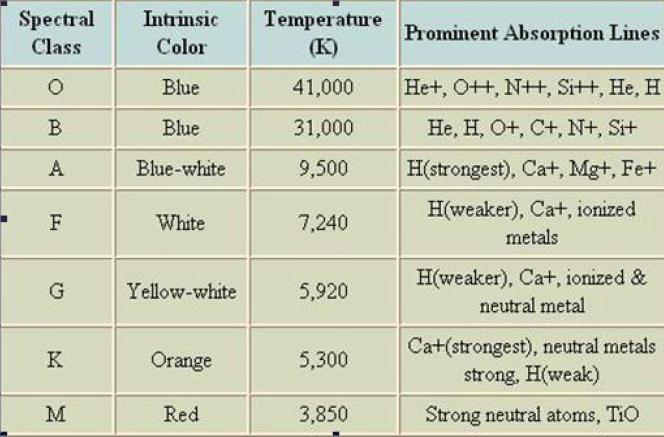
\includegraphics[angle=270,width=\textwidth]{Figures/spectral_class_table.png} 
\end{subfigure}
\begin{subfigure}[h]{0.5\textwidth}
	\centering
	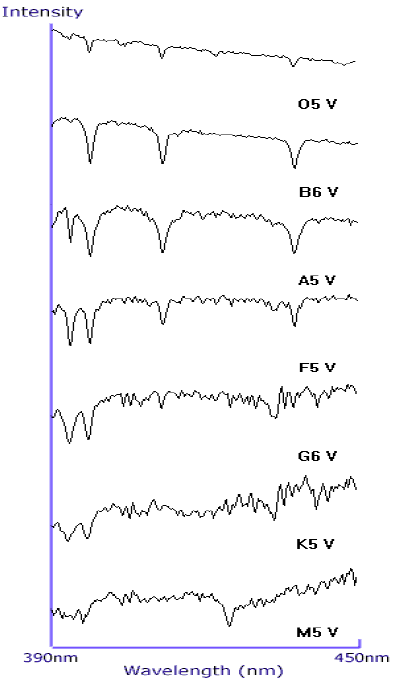
\includegraphics[scale=0.5]{Figures/spectra_comparison_harvard.png} 
    \end{subfigure}
    \caption{\textbf{Αριστερά}: Πίνακας με στοιχεία για κάθε φασματικό τύπο. \textbf{Δεξιά}: Σύγκριση φασμάτων αστέρων της κύριας ακολουθίας.}
    \label{fig:spectra_comparisson_table}
\end{figure}

Οι έξι συμπληρωματικοί φασματικοί τύποι (κόκκινα γράμματα στο σχήμα \ref{fig:spectral_classes_harvard}) περιγρέφουν μη-συνηθισμένους αστέρες. Ο τύπος W χαρακτηρίζει αστέρες τύπου \textbf{Wolf-Rayet} οι οποίοι είναι όμοιοι με αυτούς του τύπου Ο, αλλά με ευρείες γραμμές εκπομπής, οι οποίες οφείλονται σε ανώμαλα εκτεταμένη ατμόσφαιρα.
Ο τύπος P χαρακτηρίζει \textbf{πλανητικά νεφελώματα}, ένα από τα τελικά στάδια της εξέλιξης ενός αστέρα μικρής μάζας, τα οποία αποτελούνται από εξαιρετικά αραιό αέριο και σκόνη.
Ο τύπος Q ορίστηκε για την περιγραφή των φασμάτων \textbf{καινοφανών αστέρων} (novae), αστέρες που εμφανίζουν ξαφνική αύξηση της φωτεινότητάς τους κατά πολλά μεγέθη λόγω εκρηκτικής ανάφλεξης πυρηνικού καυσίμου. Αυτό μπορεί να συμβεί είτε σε διπλό σύστημα λόγω μεταφοράς μάζας από τον ένα αστέρα στον άλλον (δες Κεφάλαιο \ref{ch:Chapter7}), είτε και σε απλούς αστέρες όταν διάφοροι μηχανισμοί πρόσμιξης μεταφέρουν φρέσκο υλικό από ανώτερα στρώματα, στα στρώματα που γίνεται καύση βαρύτερων υλικών. Πάντως ο φασματικός τύπος Q χρησιμοποιείται σπάνια σήμερα.
Τέλος, οι αστέρες φασματικού τύπου R, N και S έχουν ανώμαλη χημική σύσταση, με τα φάσματα των αστέρων R και N να περιέχουν ασυνήθιστα υψηλή περιεκτικότητα σε άνθρακα (μοριακές ταινίες της ελεύθερης ρίζας CH και CN αντίστοιχα) και να ονομάζονται \textbf{αστέρες άνθρακα}. Από την άλλη, τα αστέρια φασματικού τύπου S, έχουν έντονες μοριακές ταινίες των οξειδίων του τιτανίου, ζιρκονίου και άλλων σπάνιων γαιών. Αυτη η ανώμαλη χημική σύσταση αυτών των αστέρων μάλλον οφείλεται σε κάποιον μιχανσιμό ανάμιξης της επιφανειακής ύλης με ύλη που προέρχεται από το εσωτερικό του αστέρα μέσω ρευμάτων μεταφοράς. 
Ας σημειωθεί εδώ ότι οι έξι αυτοί φασματικοί τύποι που αναλύσαμε δεν αποτελούν γνήσια επέκταση της αρχικής φασματικής ταξινόμησης, καθώς δεν παρουσιάζουν αμφιμονοσήμαντη αντιστοιχία μεταξύ των φασματικών τύπων και των ενεργών θερμοκρασιών. Τα αστέρια που ανήκουν σε αυτές ή αλλες φασματικές κατηγορίες που δεν εμφανίζονται εδώ (π.χ. L και T κατηγορίας καφέ νάνων) αποτελούν πολύ μικρό ποσοτό της τάξης $< 1 \%$.

Παρόλα αυτά, υπάρχουν αστέρια που φυσικά η ενεργός τους θερμοκρασία εμπίπτει στα όρια $ 3000 - 50000 \ K$ αλλά το φάσμα τους δεν ταιριάζει με κανέναν από τους παραπάνω φασματικούς τύπους. Γι' αυτό γενικά η χρήση της θερμοκρασίας ή του δείκτη χρώματος (που είναι συνάρτηση της θερμοκρασίας) προτιμάται έναντι του φασματικού τύπου.



\subsection{Διάγραμμα Hertzsprung-Russell}
Αν τοποθετήσουμε τους αστέρες με γνωστά φάσματα σε ένα δισδιάστατο διάγραμμα που έχει τετμημένη τον φασματικό τύπο (Sp) και τεταγμένη το απόλυτο μέγεθος του αστέρα, τότε παρατηρούμε ότι οι αστέρες δεν είναι τυχαία διασκορπισμένοι στο επίπεδο, αλλά συγκεντρώνονται σε συγκεκριμένες δομές. Το διάγραμμα αυτό ονομάζεται \textbf{διάγραμμα Hertzprung-Russel} ή για συντομία διάγραμμα H-R.
Η μορφή του διαγράμματος H-R μας δείχνει ότι υπάρχουν φυσικοί νόμοι που συνδέεουν τη λαμπρότητα του αστέρα (απόλυτο μέγεθος) με την ενεργό θερμοκρασία του (φασματικό τύπο) και ότι όλα τα βασικά παρατηρησιακά μεγέθη ενός αστέρα δεν έχουν τυχαίες τιμές, αλλά συνδέονται με σχέσεις που μπορούν να εξηγηθούν και θεωρητικά. Φυσικά μία σχέση της μορφής $$ L = f(T_{eff})$$ που αποκαλύπτει το διάγραμμα H-R είναι προσεγγιστική καθώς οι αστέρες χαρακτηρίζονται και από άλλες ποσότητες, όπως η χημική σύσταση, που σε πρώτη φάση αγνοούνται. Γι' αυτό άλλωστε και οι αστέρες δεν βρίσκονται στο διάγραμμα H-R κατά μήκος μονοδιάστατων καμπυλών, αλλά παρουσιάζουν μία κάποια διασπορά.

\begin{figure}[h]
    \centering
    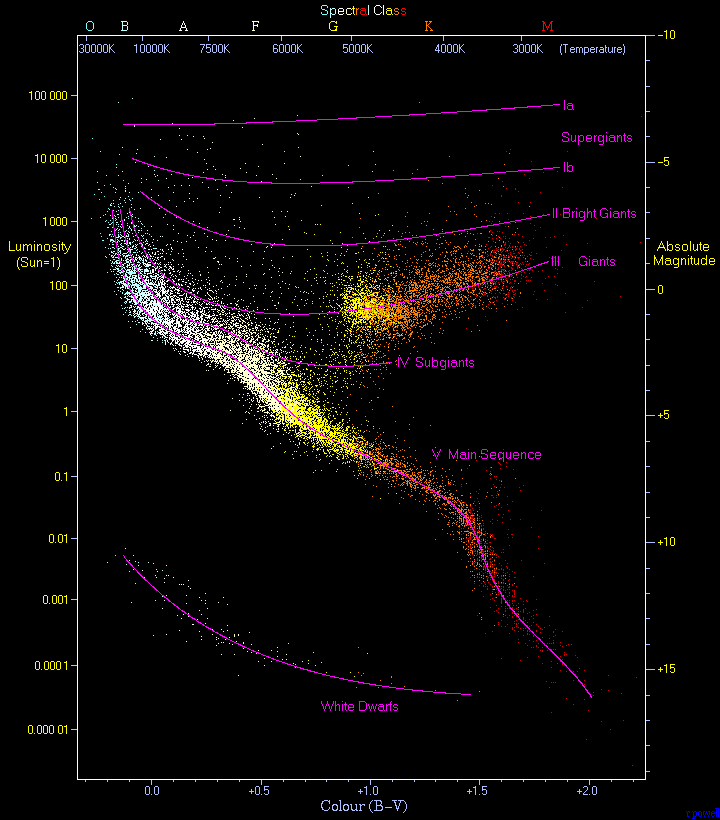
\includegraphics[scale=0.4]{Figures/HRDiagram.png}
    \caption{Διάγραμμα Hertzprung-Russel.}
    \label{fig:HRD}
\end{figure}

Από το σχήμα \ref{fig:HRD} παρατηρούμε ότι τα περισσότερα αστέρια είναι συγκεντρωμένα σε μία ζώνη, που διατρέχει το διάγραμμα διαγώνια και η οποία ονομάζεται \textbf{κύρια ακολουθία}. Πάνω από την κύρια ακολουθία υπάρχει μία άλλη ζώνη αστέρων, που ονομάζεται \textbf{κλάδος γιγάντων}. Τέλος, κάτω από τον κλάδο της κύριας ακολουθίας υπάρχει μία συγκέντρωση αστέρων, που βρίσκεται αριστερά του διαγράμματος και σε αυτή ανήκουν οι \textbf{λευκοί νάνοι}. Αν προεκτείνουμε την γραμμή του κλάδου των γιγάντων προς τα αριστερά, παρατηρούμε ότι τέμνει την κύρια ακολουθία σ' ένα σημείο που αντιστοιχεί περίπου στον φασματικό τύπο A0 και απόλυτο μέγεθος $ M = +1$. Οι αστέρες που βρίσκονται αριστερά από το φασματικό τύπο Α0 ονομάζονται αστέρες \textbf{προγενέστερου φασματικού τύπου} (π.χ. κυανοί γίγαντες), ενώ οι αστέρες που βρίσκονται δεξιά από τον φασματικό τύπο Α0 ονομάζονται αστέρες \textbf{μεταγενέστερου φασματικού τύπου} (π.χ. ερυθροί νάνοι, νάνοι της κύριας ακολουθίας κτλ). Οι αστέρες μεταγενέστερου φασματικού τύπου που βρίσκονται πάνω από την κύρια ακολουθία ονομάζονται \textbf{ερυθροί γίγαντες}. Η διάκριση των αστέρων σε αστέρες προγενέστερου και μεταγενέστερου φασματικού τύπου δεν έχει σήμερα καμία άλλη σημασία παρά μόνο την περιγραφή της θέσης τους στο διάγραμμα H-R. Αντίθετα, η διάκριση των αστέρων σε νάνους και γίγαντες έχει φυσική σημασία.

\textbf{Αστρικά σμήνη}\\
Μπορούμε να διακρίνουμε δύο ειδών αστρικών σμηνών. Τα \textbf{σφαιρωτά σμήνη} είναι πυκνές συγκεντρώσεις μεγάλου αριθμού αστέρων ($10^4 - 10^6$) με σφαιρικό σχήμα, που κινούνται σε ελειπτικές τροχιές στην άλω γύρω από το κέντρου του Γαλαξία. Το χαρακτηριστικό των σφαιρωτών σμηνών είναι ότι επειδή σχηματίστηκαν από την βαρυτική κατάρρευση του ίδιου μοριακού νέφους, αποτελούνται σε πρώτη προσέγγιση από άστρα της ίδιας χημικής σύστασης (ίδια ``μεταλλικότητα''), της ίδιας ηλικίας, και βρίσκονται στην ίδια απόσταση από τη Γη.
Η άλλη κατηγορία αστρικών σμηνών είναι τα \textbf{ανοικτά σμήνη} τα οποία είναι συγκεντρώσεις το πολύ μερικών χιλιάδων άστρων που σχηματίστηκαν και αυτά από το ίδιο μοριακό νέφος, αλλά τα αστέρια είναι πληθυσμού I, και άρα πολύ νεώτερα συγκριτικά με τα αστέρια στα σφαιρωτά σμήνη που είναι πληθυσμού ΙΙ. Τα ανοικτά σμήνη βρίσκονται κυρίως στο Γαλαξιακό επίπεδο και όχι στην άλω.


\begin{figure}[h]
    \centering
    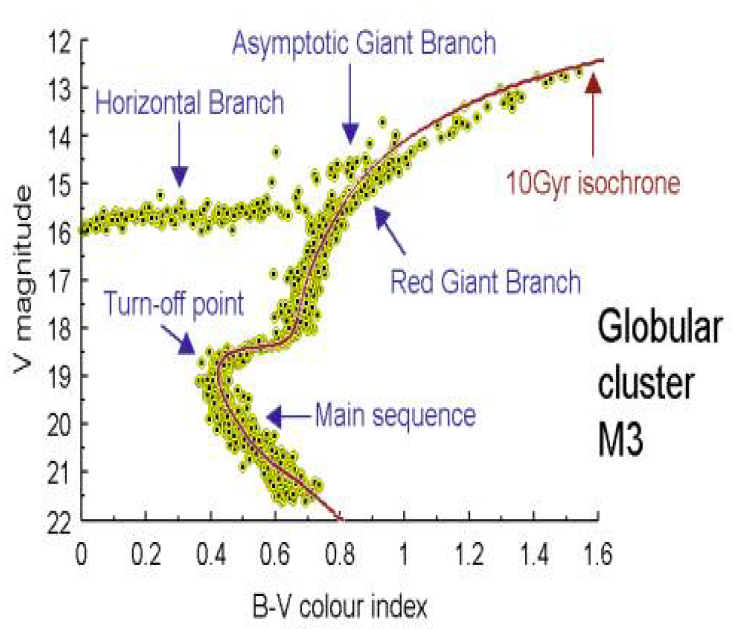
\includegraphics[scale=0.4]{Figures/cmd.png}
    \caption{Διάγραμμα Χρώματος-Μεγέθους για το σφαιρωτό σμηνος Μ3. Στο διάγραμμα φαίνεται μια ισόχρονη καμπύλη των 10Gyr.}
    \label{fig:CMD}
\end{figure}

Είναι προφανές ότι δεν μπορούμε να πάρουμε το φάσμα για κάθε ένα από τα αστέρια-μέλη ενός σμήνους. Γι' αυτό το λόγο, όταν θέλουμε να κάνουμε το διάγραμμα H-R στην περίπτωση σμήνους αστέρων, εκφράζουμε την τετμημένη σε όρους δείκτη χρώματος (που είναι συνάρτηση της θερμοκρασίας και μπορεί να υπολογιστεί για χιλιάδες αστέρια που βρίσκονται στο ίδιο οπτικό πεδίο) αντί για φασματικό τύπο, και την τεταγμένη σε μέγεθος αντί για λαμπρότητα. Έτσι προκύπτει το λεγόμενο \textbf{διάγραμμα χρώματος-μεγέθους} (color-magnitude diagram) που φαίνεται στο σχήμα \ref{fig:CMD}.

Αν η συνάρτηση αρχικής μάζας (initial mass funtion) ενός σμήνους είναι γνωστή, τότε μπορούμε να υπολογίσουμε θεωρητικά μια ισόχρονη καμπύλη για οποιαδήποτε ηλικία θέλουμε, με το να προσομειώσουμε την εξέλιξη του κάθε αστέρα του αστρικού πληθυσμού και κάνοντας το διάγραμμα H-R για αυτά τα αστέρια. Συγκρίνοντας τις θεωρητικές αυτές καμπύλες που αντιστοιχούν σε συγκεκριμένες ηλικίες με το παρατηρησιακό διάγραμμα χρώματος-μεγέθους, μπορούμε να έχουμε μία εκτίμηση για την ηλικία του σμήνους.





\subsection{Ταξινόμηση κατα Yerkes}
Αστέρια ίδιου φασματικού τύπου (ίδιας ενεργού θερμοκρασίας) εμφανίζουν κατανομή στις λαμπρότητές τους, όπως φαίνεται και από το διάγραμμα H-R (σχήμα \ref{fig:HRD}). Για παράδειγμα, ο εγγύτατος του Κενταύρου έχει την ίδια επιφανειακή θερμόκαρσία με αυτή του Betelgeuse, άρα ανήκουν στον ίδιο φασματικό τύπο, αλλά τελείως διαφορετικές λαμπρότητες με τον εγγύτατο να έχει 100 φορές μικρότερη λαμπρότητα από τον Ήλιο και τον Betelgeuse 100,000 φορές μεγαλύτερη λαμπρότητα.

Το 1930, οι Morgan \& Keenan, πρότειναν ένα νέο σύστημα ταξινόμησης των αστέρων, το οποίο λειτουργεί συμπληρωματικά του συστήματος ταξινόμησης κατα Harvard. Το νέο σύστημα βασίζεται στην έννοια της \textit{Κατηγορίας λαμπρότητας}. Σύμφωνα με αυτή την ταξινόμηση, αστέρια της \textbf{ίδιας} ενεργούς θερμοκρασίας (ίδια φασματική τάξη), χωρίζονται σε έξι κατηγορίες λαμπρότητας, με βάση το \textbf{πλάτος} των γραμμών απορρόφησης (σχήμα \ref{fig:spectral_classes_yerkes}).

\begin{figure}[h]
   \centering
\begin{subfigure}[h]{0.42\textwidth}
	\centering
   	 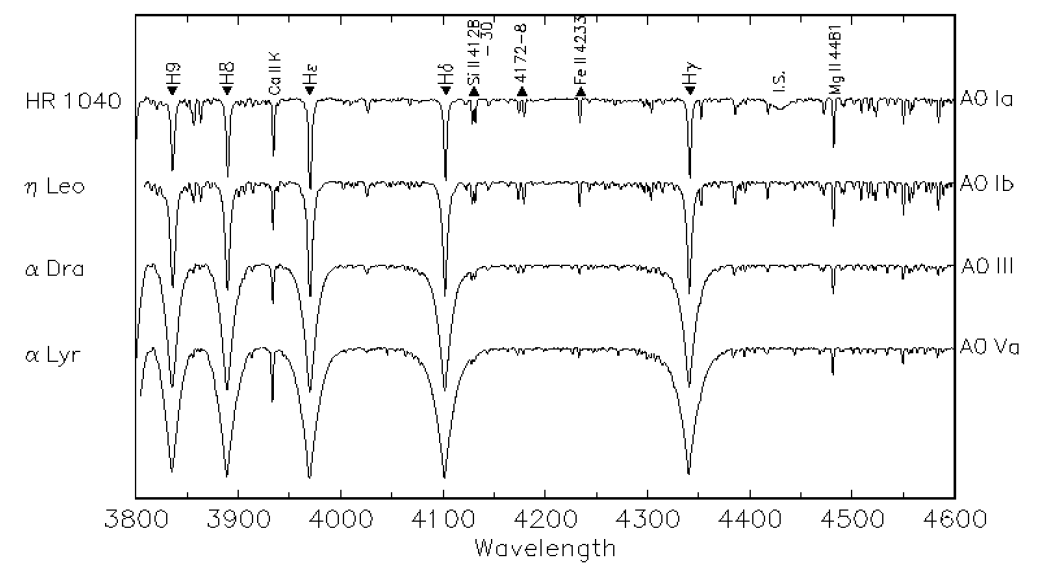
\includegraphics[angle=270,origin=c,scale=0.3]{Figures/luminosity_variations_yerkes.png} 
\end{subfigure}
\begin{subfigure}[h]{0.55\textwidth}
	\centering
	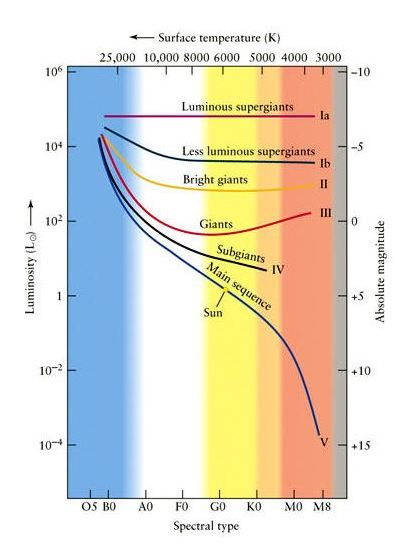
\includegraphics[scale=0.6]{Figures/spectral_classes_yerkes.jpg} 
    \end{subfigure}
    \caption{\textbf{Αριστερά}: Διακύμανση του πλάτους των γραμμών απορρόφησης για τέσσερια αστέρια φασματικού τύπου Α0 (HR 1040, $\eta$ Leo, $\alpha$ Dra, $\alpha$ Lyr). \textbf{Δεξιά}: Φασματική ταξινόμηση κατά Yerkes, σε έξι κατηγορίες λαμπρότητας. Για μεγαλύτερη κατηγορία λαμπρότητας ($ I, II, \dots VI$) το πλάτος της γραμμής απορρόφησης αυξάνεται, ενώ η ακτίνα και η λαμπρότητα μειώνονται. Ο Ήλιος ανήκει στην κατηγόρια G2V.}
    \label{fig:spectral_classes_yerkes}
\end{figure}

\vspace{0.5cm}
{\color{red} \hrule}
\textbf{Ερμηνεία της κατάταξης κατά Yerkes}\\
Εφόσον μιλάμε για αστέρια ίδιου φασματικού τύπου, το εύρος της γραμμής απορρόφησης δεν οφείλεται σε διαφορές στην ενεργό θερμοκρασία (ούτε στην περιστροφή των αστέρων) αλλά στην πίεση στην επιφάνεια των αστέρων. Κάνοντας μερικές απλές παραδοχές, μπορεί να δειχτεί ότι η ατμοσφαιρική πίεση σε έναν γίγαντα αστέρα είναι μικρότερη από την πίεση σε έναν νάνο αστέρα. Συνδυάζοντας αυτό το αποτέλεσμα με τον νόμο του Saha που μας δίνει τον βαθμό ιονισμού ενός αερίου, μπορούμε να εξηγήσουμε τις φασματικές διαφορές ανάμεσα σε αστέρια του ίδιου φασματικού τύπου.\\
{\color{red} \hrule}

